% !TeX spellcheck = en_US
\documentclass[sigconf]{acmart}

\usepackage{booktabs} % For formal tables
\usepackage{graphicx}
\graphicspath{{./images/}}
\usepackage{float}
\usepackage{amssymb}
\usepackage{booktabs}

% Copyright
%\setcopyright{none}
\setcopyright{rightsretained}

%Conference
% \acmConference[WOODSTOCK'97]{ACM Woodstock conference}{July 1997}{El
%   Paso, Texas USA} 
% \acmYear{1997}
\copyrightyear{2017}


\begin{document}
\title{Personalized music search based on graph embedding}


\author{Christian Esswein}
\affiliation{%  
  \institution{Databases and Information Systems}
  \department{Department of Computer Science}
  \state{University of Innsbruck} 
}
\email{christian.esswein@student.uibk.ac.at}


\begin{abstract}
	While exploring new music, users are typically limited to recommender systems which are proposing items either based on their listening history or on content similarities. Combining both methods models a "query-based recommendation" which enables users to filter content based on their preferences.
	The ecosystem of music can be represented as an heterogeneous graph using all available data like tracks, artists, genres, tags and users. Using graph embedding techniques a low-dimensional vector representation is learned and provides a simple method to calculate similarities. Search queries, either single terms or combinations of items in the music graph, can be encoded using the same vector space. Therefore, not only exact results are found, but also similar items.
	
	This work presents an approach to create a music search with Spotify data where new users can connect with their existing accounts. The retrieved results are not only presented in a list but instead the learned vector representation is exploited to generate 3D representations.
\end{abstract}


\keywords{Recommender Systems, Graph Embedding, Personalization}

\maketitle

\section{Introduction}
In recent years music streaming platforms are getting more popular which enables users to access huge collections of music. With this trend it has also changed how users search and explore music~\cite{lee2016look}. For example Spotify\footnote{\url{http://www.spotify.com}} with currently 140 million active users has over 30 millions songs to offer (as of June 2017)~\cite{aboutSpotify}. As a consequence of this huge collection of songs, the primary objective for user is not to find specific songs anymore but to find songs matching seeding criteria. 
While exploring new music, users are typically limited to recommender systems which are proposing items either based on their listening history or on content similarities (aka find similar artists, songs). Combining both methods models a "query-based recommendation" which enables users to filter content based on their preferences.

When using naive approaches with simple attribute matching queries, complete annotated metadata is required. Otherwise songs can not appear when querying for tags which they are not assigned to. Especially when it comes to genres and tags for tracks it is unfeasible to manually annotate every entity. A desired search engine needs to learn the representation with some tags in the training phase but while predicting new connections have to be drawn.
The ecosystem of music can be represented as an heterogeneous graph using all available data like tracks, artists, genres, tags and users. Using graph embedding techniques a low-dimensional vector representation is learned and provides simple method to calculate similarities. Search queries, either single terms or combinations of items in the music graph, can be encoded using the same vector space. As a result, not only exact results are found, but also similar items. \\

This work presents an approach to embed the Spotify dataset into a latent representation to enable recommendations based on queries. After providing the first search results, the user should be assisted while exploring the remaining items and in the refinement of his search terms. Traditional list based aggregations of search results can only model a one dimensional view for the items. Instead of a list, the low-dimensional vector representation should be exploited to generate 3D representations of the suggested items. Combined with the graph representation, query suggestions can be provided.

% Additionally the assignment of scores is a hard task --> how to compare. having / not having. Approaches try to predict tags through audio features -> lack to compare different seeds. how to compare artists with tracks


\section{Related work}

In \cite{chen2016query} a very similar approach is presented where query-based music recommendations are created with embedded graphs. The main difference is that the music graph was modeled as a bipartite graph with users in one and all other items in the other set. This allows to create next track recommendations based on recent seed tracks but does not model a full qualified search because music items themselves are not connected. 

To evaluate the performance of my query recommendations, playlist names are used to predict their tracks. On the same dataset \cite{chungexploiting} presented a text-based method to embed and query for tracks. Here similarities between items are only based on co-occurring songs. \\

Alternative representation and exploration models for music are mainly complex and require additional hardware. \cite{lamere2007using} presented a 3D interface to visualize similarities between tracks. Each item is represented as a single item but no clusters are used and album covers are only involved in separate visualizations. The music space is mapped on a virtual landscape in \cite{knees2007exploring} which makes it possible to observe audio based similarities and clusters but the interface is rather complex.

\section{Graph Embedding}
Graph embedding techniques aiming to transform graph structures into low a dimensional vector space. More formally, given a graph $ G = (V,E) $ with vertices $ V $ and edges $ E $ "a graph embedding is a mapping $ f : v_{i} \rightarrow y_{i} \in \mathbb{R}^{d} $ $ \forall i \in [n] $ such that $ d \ll |V| $ and the function $ f $ preserves some proximity measure defined on graph $ G $"~\cite{goyal2017graph}. The final result is therefore a vector representation of each node in the initial graph. Having this coherent search space makes it much easier to calculate higher-order proximities between heterogeneous nodes. Similar items can be retrieved using nearest-neighboring searches.

Existing embedding algorithms can in general be categorized into factorization based, random walk based and deep walking based methods. Concerning time complexity and preserved higher order proximities, mainly random walk based methods are interesting. Others methods either only embed similarities between connected nodes or their runtime is dependent on the number of edges in contrast to $ O(|V|) $~\cite{goyal2017graph}. Short random walks over edges are used to generate sentences which reflect the graph structure. Using this walks as training data, a representation for each word is learned. In the field of natural language processing this method is known as word embedding and especially popular with \emph{Word2vec}~\cite{mikolov2013efficient}. Both \emph{Deepwalk}~\cite{perozzi2014deepwalk} and \emph{node2vec}~\cite{grover2016node2vec} are making use of \emph{Word2vec} in their reference implementations to embed arbitrary graph structures with random walks. For this work \emph{Deepwalk} was chosen because despite that \emph{node2vec} retrieves better embeddings in theory, it is not possible to extend the graph structure after its initial creation as explained in the next section.

\subsection{Model extension}
In real world scenarios, the dataset is not fixed and during runtime, more data is collected which needs to be included into the model. New data can either consists of new edges, e.g. new listening events of users during the use of the system, but also of new vertices when tracks or users are added. Especially if new users do not suffer from the cold start problem because initial data is available (e.g. through connecting with other services, see \ref{sec:impl_spotify_connect}), a fast method is desirable such that the system can be used right away. A naive approach could simply recreate the whole embedding, but this is not scalable for bigger sets. 

Random walk based embedding techniques are mostly online algorithms which can consume new walks as they are produced. This property is very powerful in general because for huge datasets not all walks have to be generated in advanced or even kept in memory. Unfortunately, both reference implementations for \emph{node2vec} and \emph{DeepWalk} do not provide interfaces to store the internal state, retrieve intermediate embeddings or continue learning. Even worse, such interfaces could only improve node proximities performance through adding edges. In order to be able to include new vertices, the internal data structures must be extended. For \emph{node2vec}, such an extension is not possible because the probability distribution of random walks is not uniform and precomputed before walk generation. For doing this, the whole graph has to be known and no graph structure can be added afterwards because it would invalidate previous transition probabilities.

% TODO:_eva explain computatinoal model
However, \emph{DeepWalk} uses a uniform distribution over random walks and as previously noted, uses \emph{Word2vec} to compute the actual embedding. Using  \emph{Word2vec} in the backend makes it possible to store the current computational model and later restore it for further learning and additionally also allows to extend the current vocabulary, in this case adding new nodes, during runtime. Together the desired options are available to partially extend the existing graph and retrieve the new embedding.

To extend an existing embedding, first, new vertices and edges have to be collected and appended to the existing graph. Then new random walks are generated, but only over added vertices and edges. This new training data has only a small size compared to the initial data set and is proportional to the number of added structure. Then finally the existing \emph{Word2vec} model can be loaded, extended with new nodes, and learning is continued with new walks. \\


% Scalability:
With this method, graph and embedding can be updated with much less effort than relearning the complete model. Even small changes can influence the whole embedding and create a new vector space. The scalability is therefore questionable because for big datasets the new embedding has to be updated completely which may invalidate all created indexes. Furthermore only graph structure can be extended but not modified or removed.

% TODO: check percentage when adding node...
% TODO: compare time between initial learning and extending: 3mins extending, 30min full model

\section{Personalized queries}
The increasing availability of huge music datasets through streaming platforms requires more sophisticated search methods to access desired tracks. Especially on streaming platforms, users expect to filter and consume music with predefined seeds like genres, context based scenarios or queries to find similar items of "x". This content based filters are in contrast to personal recommendations which are only based on historic listening behavior. To combine those two concepts and to allow users to specify arbitrary search intention, a flexible query system is required.

The music corpus can be modeled in a heterogeneous graph with tracks, artists, album and tags as nodes and relationships as edges. Using graph embedding techniques as described in the previous section, a vector space with preserved proximities is created. Each item from the graph is included in the final embedding and can therefore be used as query term. Nearest neighbors represent similar items with decreasing confidence on higher distances. Because every query is formulated with vectors, also the combination of different search terms is possible. The retrieved items have mixed item types which means that not only tracks are returned but also artists for example. This is very powerful because neither user nor system have to decide at first hand the item type but can also easily apply filters. Another benefit is, that similarity measures between different item types are possible.

It is crucial to include as many graph structure as possible to produce meaningful outputs. Tracks together with connected artists for example are clearly too sparse, mainly because no edges between different tracks or artists exist. Including tags for tracks and genres for artists does solve two problems. On the one hand side, it models similarities between different items and therefore improves the embedding. On the other hand, it enriches the possible terms which can be used by users to construct queries. \\

Until now the user itself was not included into the system. If user feedback is available, e.g. through historic track listening behavior or positive feedback on items, this data can be included into the graph. This improves the available graph structure and therefore may improve the embedding quality and additional makes it possible to model a user preference on queries. For each user initiated search query, the user context is added and influences results with personal recommendations. Using the user without additional seed items even retrieves general recommendations with the same system.

% add query definition with math syntax?

\subsection{Search refinement}
% TODO: cite...

% extend query
Searching for music is not a single action process where a user formulates query intention and then consumes the results. The search can be seen as a process where query refinements are always part of it. Therefore it is necessary that users are not only able to extend queries but also are supported with suggested terms. The user should feel like navigating through a virtual result space instead of jumping to unconnected places after manually modifying requirements. Having a search query which is represented as a vector, it can partially constructed as a combination of multiple search term vectors. This means that any of the proposed items can be used to further extend the query and refine the search.

For example suppose that you first search for a music genre you are interested in and then find an artists in the results which matches your search intention. Adding this artist to the current query will not limit new results to the added artists but will return items which are similar to the genre and artist. Using this technique the user has not actively adapt the query through reformulating it and still gets more precisely results. \\

\subsection{Result representation and exploration}
% TODO: cite...

% 3D
The most common visualization for recommendations is a list of items which is ordered by relevance for the user. Only the ordering can be observed and therefore it represents a very limited one dimensional view where even distance measures between consecutive items are not visible. To create at least a sense of vision for distances to the most significant items, it is common to spread the results among multiple result pages. 
When having an embedding where similarities between arbitrary items can be expressed using vectors, more advanced interfaces are possible. Using dimension reducing methods like the Principal component analysis (PCA), the embedding can be compressed to three dimensions. Instead of using a list, the retrieved recommendations items can then easily visualized in a 3D scene. Each track, artist or album has a corresponding position vector and is representable as interactive 3D object. Using such an interface does not only express distance measure between items but also allows the user to explore the result space more easily. Less accurate items are positioned around the center hit and the direction in three dimension can be chosen to explorer additional items. This means that the query itself is refined while exploring the result space indirectly and without active user involvement.

Similar items are positioned very nearby and when applying distance based clustering, accumulations of items can be represented as single but annotated clusters. For exploration, only one item has to be inspected for deciding whether the whole cluster is in interest or not. Postfiltering to remove variants of very similar items is then not necessary anymore while all items are still available. Additionally this also simplifies the visualization because more items can be displayed on less space without introducing noise.\\

It is crucial to simplify the inspection of single items such that big collections are explorable in reasonable time. Album covers as textures for 3D objects improve the vision because known items can be recognized and the discovery or desired tracks is more efficient~\cite{libeks2011you}. To provide detail information about selected items (e.g. artist name for track, genres), directly connected neighbors can be retrieved from the initial graph structure. Finally music samples have to be provided to rate and consume discovered tracks. \\

Through advantages in browser technology just in time visualizations of 3D scenes can be created directly on websites without complex precomputations or add-ons. Also users are nowadays more familiar with interactive and multidimensional interfaces. Enhanced result views could therefore may replace simple lists.

\section{geMsearch}
\emph{geMsearch} is a prototype which implements the proposed method for personalized music search. An embedded music corpus is searchable through a web client and retrieved items are represented in a list or 3D view which can be seen in figure \ref{fig:web_client} and \ref{fig:web_client_3d}. Besides the offline evaluation this makes it possible to test the implementation in a real world scenario. 

Supported with autocomplete suggestion the user can select any item of the graph to formulate single or combined queries. To provide recommendations, this selection is send to the API server instance and evaluated on the embedded graph. User filters can further restrict the search results for certain element types, like tracks, tags or artists. Before sending results to the client, additional metadata like artist names for tracks and album covers are queried from a simple document store and added to the response. Because of its popularity and easy to use API the data highly depends on the Spotify API. This ensures a high availability of metadata as well as album covers and makes it possible to play short sound samples for each track.\\

\begin{figure}[ht]
	{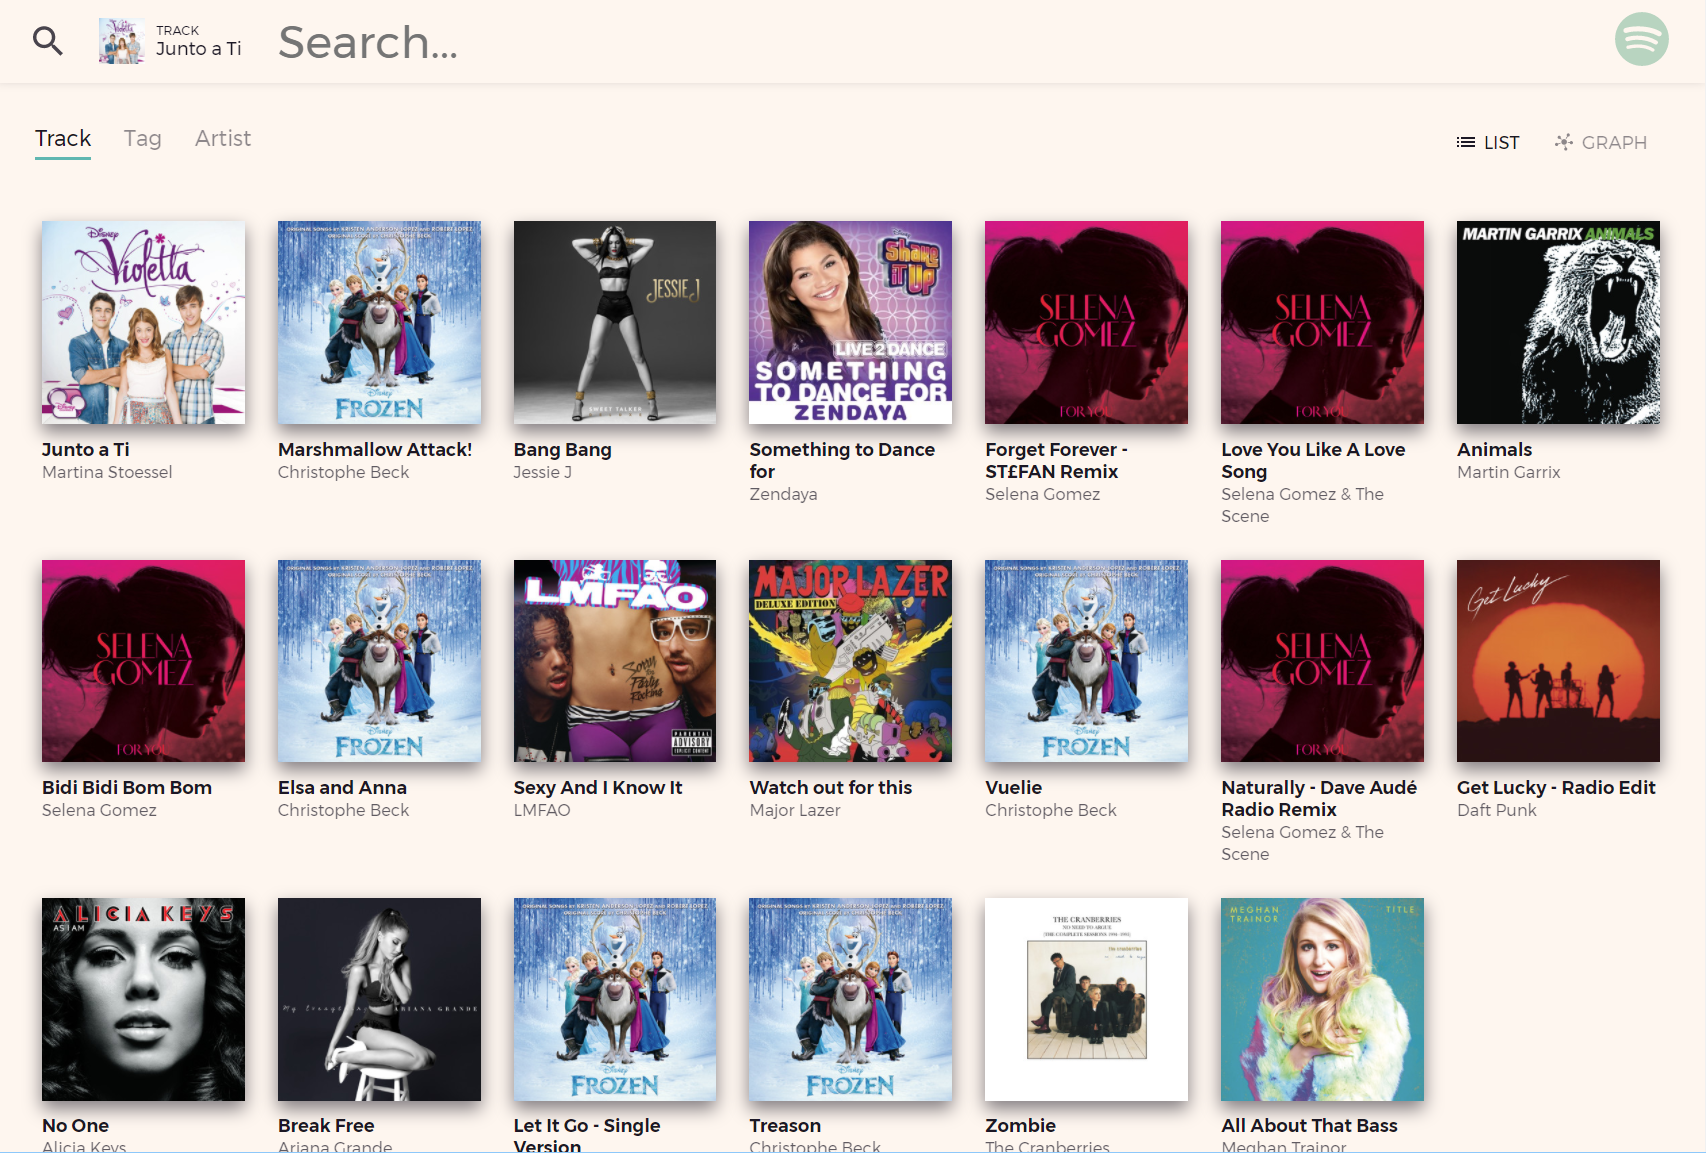
\includegraphics[width=250px]{web_client.png}}	
	\caption{Web client list results}
	\label{fig:web_client}
\end{figure}

\begin{figure}[ht]
	{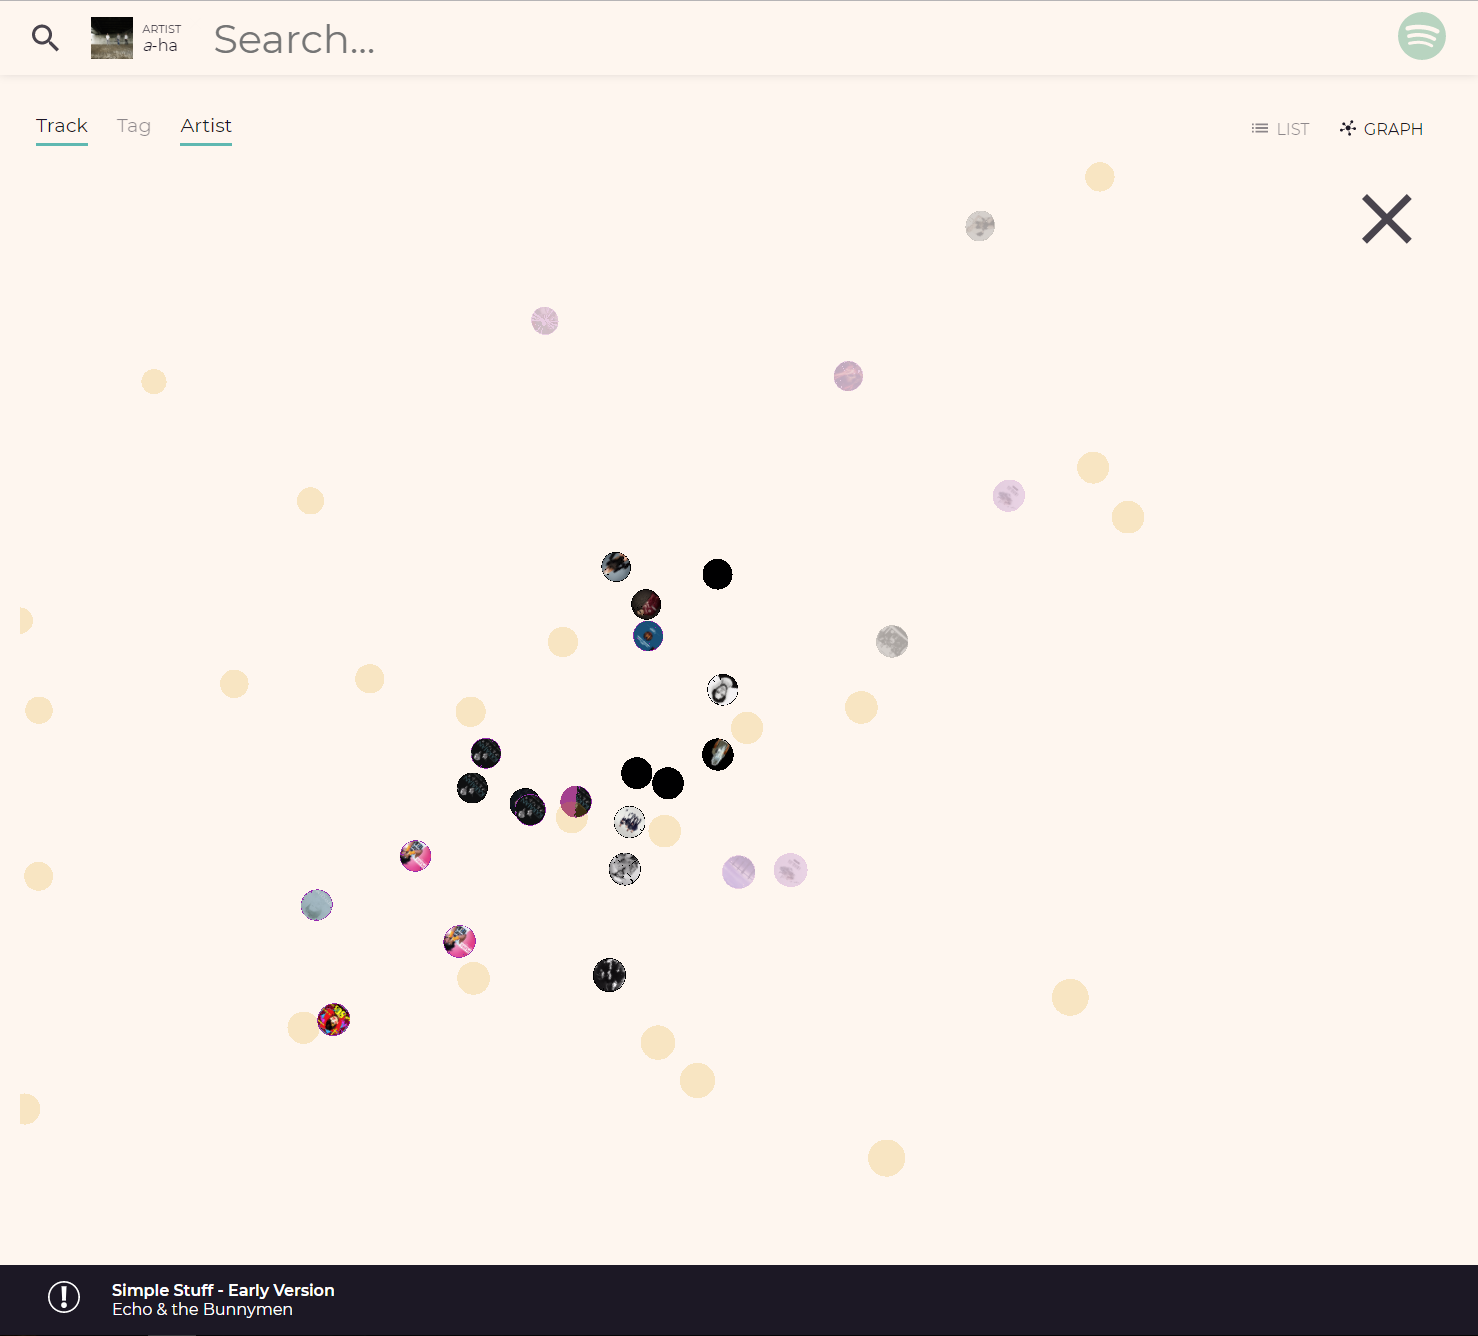
\includegraphics[width=250px]{web_client_3d.png}}	
	\caption{Web client 3D view and player bar}
	\label{fig:web_client_3d}
\end{figure}

% \subsection{Spotify connect}
\label{sec:impl_spotify_connect}
To overcome the cold start problem for user profiles and making the client usable, users can connect with their Spotify account. The official Spotify API supports the OAuth protocol with different scopes which makes it possible to access personal playlists, playing history and saved tracks. To create a personal preference profile, \emph{geMsearch} only accesses the saved tracks because it requires much less preprocessing and computational effort than the whole playing history which is potential very big and contains much more noise. After a user has connected with his account, the music library is loaded and compared with known tracks in the current database. Missing songs are crawled to include metadata from Spotify about the track and artist, as well as user curated tags from Last.fm. After this data is collected, the graph can be extended and included into the existing embedding.

This approach can only recommend and present known items in the database which clearly does not reflect all tracks from Spotify. The initial model is pretrained and evaluated with playlists as discussed in the next section and with every user this dataset is extended and improved.

\section{Experiments}
Estimating the quality of the presented approach is one of the key challenges because there exist no dataset which directly maps search queries with user context to results. Even having a working prototype client to test the system on real users, representative user studies require fairly big and diverse users bases. The test cases need to allow the users to estimate the results without being biased through available options or the test environment. A/B tests can model fair and solid results but require scopes in terms of number of users and participation which are only available on commercial platforms. Therefore, the common approach in research is to make use of crawled playlists which were manually created by users. As presented in \cite{kamehkhosh2017user}, this evaluations are comparable to user studies but require much less effort. Additionally, offline experiments can be easily repeated with adapted implementations and input parameters which helps during implementation and optimization to observe and benchmark the outcome. \\

Manually curated playlists can easily obtained, they have an user context and are usually labeled with a name. In a broader sense the contained tracks can therefore be seen as the desired output for queries by the name, related to the user. This is why the \emph{playlist evaluation}, further described in section \ref{subsec:playlist_eval}, uses the playlists as ground truth and tries to predict the tracks based on user context and playlist name. To evaluate the embedding quality in respect to personal preferences the \emph{track recommendation evaluation} in section \ref{subsec:track_rec_eval} compares user track recommendations to baseline methods.


\subsection{Dataset and graph generation}
The initial dataset was constructed from a crawled Spotify playlists by DBIS at the University of Innsbruck~\cite{pichl2017improving}. This data consists of playlists with an user context and contained tracks with artist and audio features. In order to enrich the available query terms and gather more graph structure, social curated track tags were crawled from \emph{Last.fm} \footnote{\url{https://www.last.fm/api/show/track.getTags}} and artist genres from Spotify.
%  \emph{Last.fm}\footnote{\url{www.last.fm}}

Because both the playlists and the \emph{Last.fm} tags where unfiltered user produced data, in a preprocessing was necessary. All playlists with less than four tracks or names without an alphanumeric title are removed. Within the dataset 12 tracks are most common in a playlist. To match same tags on different tracks, the names are transformed to lowercase and special characters are removed. Tags with less than four characters, or without more than five user assignments on a given track are also cleaned.

Table \ref{table:node_count} and \ref{table:edge_count} show which and how many elements and connections are contained in the graph after preprocessing.

\begin{table}[H]
	\caption{Node count by type:}
	\label{table:node_count}
	\begin{tabular}{lr}
		\midrule 
		\textbf{Type} & \textbf{Count} \\ 
		\midrule 
		Playlists & 21,336  \\
		Users     & 1,180     \\
		Tracks    & 852,293 \\
		Artists   & 110,377  \\
		Tags      & 395,587    \\
		Albums    & 189,174    \\
		Genres	  & 1,520	\\
		\midrule 
		Total nodes & 1,571,467\\
		\bottomrule
	\end{tabular}
\end{table}

\begin{table}[H]
	\caption{Edge count by types (undirected):}
	\label{table:edge_count}
	\begin{tabular}{lr}
		\midrule 
		\textbf{Type} & \textbf{Count} \\ 
		\midrule 
		Playlist-User   & 21,323  \\
		User-Tracks     & 1,662,605     \\
		Track-Album		& 852,293 \\
		Track-Artists   & 1,027,918 \\
		Track-Tags   	& 9,341,603 \\
		Artist-Genre	& 148,705  \\
		\midrule 
		Total edges 	& 13,054,447\\
		\bottomrule
	\end{tabular}
\end{table}

\subsection{Playlist evaluation}
\label{subsec:playlist_eval}
To predict playlist tracks based on the playlist title, two steps are required. First a query must be constructed from the title and then this query can be used to retrieve recommendations. For the query extraction, contained terms are matched against known ones in the database. 
 
 To evaluate the performance the information retrieval measurements precision@k and recall@k are used.

problems: many names are noisy and do not describe content in any sense. results are compared with random predictor.


% TODO: elastic search is used to tranform text into queries.
--> Query expansion

% TODO: table with results

% TODO: different methods for quering + query extraction

% TODO: influence of embedding parameters: number of walks + dimensions


% todo: describe that many playlists only contain one artist because for spotify it is usual to be able to synchronize offline on mobile devices. Only text-based approaches are therfore much more powerful but do not reflect desired result. For music discovery mixed artists are much more powerful.

% TODO: multi artist test

\subsection{Track recommendation evaluation}
\label{subsec:track_rec_eval}
Queries are constructed using seeding elements combined with user context. Without seeds, the user alone can be used to query for recommendations. To perform a classic evaluation on user track recommendations, the playlists were used to construct historic track listening data, which is split into a training and test set. Using the training data, a new graph is generated and embedded. Then the users of the test set are used as queries to retrieve nearest neighbors in the embedding and compared with test tracks. To measure the performance precision@10 and recall@10 are computed and compared against baseline scores using \emph{MyMediaLite}~\cite{Gantner2011MyMediaLite}. Without personal context, the \emph{Random} method returns random items whereas the \emph{MostPopular} returns tracks with most listening counts. \emph{UserKNN} uses k-nearest neighbors based on user-based collaborative filtering. 

% TODO: table with results


% TODO: describe results

\begin{table}[H]
	\caption{Track recommendation results:}
	\label{table:track_rec_results}
	\begin{tabular}{lrr}
		\midrule 
		\textbf{Recommender} & \textbf{Precision@10} & \textbf{Recall@10} \\ 
		\midrule 
		UserKNN   & 0,02 & 0,02  \\
		geMsearch   & 0,02 & 0,02  \\
		MostPopular   & 0,02 & 0,02  \\
		Random   & 0,02 & 0,02  \\
		\bottomrule
	\end{tabular}
\end{table}

As expected, the more structural data is available the better the results perform, both for the \emph{playlist evaluation} and \emph{track recommendation evaluation}.

\section{Conclusion}
This work presented an approach to use graph embedding techniques to create a low dimensional vector space of music data. This embedding is used to create query-bases music recommendations and evaluated against playlist track predictions. Combined with a 3D representation of the result item it improves the way how user find and explorer new music. 
This method is not limited to music and may be also used in different domains where application data can be represented as graph but metadata for single items is sparse.

There is still potential for future work in order to improve the embedding itself and also the query mechanism. Weighted graphs seemed to be a promising approach to improve the embedded proximities in early tests. It could also be possible to even include audio features as graph nodes.


\bibliographystyle{ACM-Reference-Format}
\bibliography{bibtex}


\newpage
\appendix
\section{Implementation Details}


Evaluation:
in Pyhton
Graph is generated, embedded 


ElasticSearch for autocomplete im client and query extraction for playlist evaluation

MongoDb as a document store for metadata in order to enrich search results. User data is also stored here


Client
written in TypeScript to have static type checking and advanced autocomplete suggestions in editor
React with Redux 
ThreeJs to render 3D scene


explain spotify connector:
having two microservices besides API to not block resources with long running tasks for further requests. 
Crawler: Watches DB for new tracks through music library sync and makes sure that all neccessary metadata is available. For new tracks spotifiy track data and artists are crawled, then tags are retrieved from Last.fm.

Embedder: Waits until crawlers are finished and then extends existing graph with new data. The changes are collected and then existing model is retrained to retrieve new embedding which then replaces existing.



\end{document}
